\chapter{Preliminares}
\label{chapter:preliminaries}

En este capítulo se explican los conceptos básicos para
el desarrollo del proyecto, separados en secciones.
El tema principal son los algoritmos genéticos, 
además de esto se explican de manera detallada los conceptos que se
tomarán en cuenta en el desarrollo de los métodos que componen el sistema,
siendo estos: open-ended evolution, generación procedural de contenido y los
conceptos básicos de jugabilidad.

\section{Algoritmos Genéticos}
\label{section:genetic-algorithms}

Los algoritmos genéticos (Genetic Algorithms, GAs por sus siglas en Inglés) son
algoritmos inspirados en la evolución Darwiniana y utilizados para la
optimización de procesos, fueron propuestos por John Holland en 1975
\cite{Holland1975}, los GAs son métodos de optimización y búsqueda basados en los
principios de la selección natural y genética, la manera de representarlos es
mediante un grupo de individuos que representan posibles soluciones a un
problema y mediante el uso de operadores genéticos estos individuos se cruzan y
evolucionan para acercarse más al objetivo, el cual puede ser minimizar o
maximizar una función de utilidad para un sistema.

De acuerdo a una explicación proporcionada por Whitley en uno de sus artículos
\cite{Whitley1994}, un algoritmo genético (GA) es un algoritmo de optimización
inspirado en el proceso natural de evolución. Por esta razón los GAs son
considerados como parte de una subárea de algoritmos de optimización llamada
algoritmos evolutivos. La manera en cómo funciona un GA es que se propone tener
un conjunto inicial de posibles soluciones al problema, estas soluciones son
llamadas población dentro del algoritmo. Cada una de estas soluciones propuestas
llevan el nombre de individuos y en ocasiones se definen como cromosomas. Esta
población es evaluada mediante el uso de una función de aptitud encargada de
determinar el rendimiento de cada uno de los individuos como una de las posibles
soluciones para el problema que se está tratando. Este tipo de problemas
comúnmente involucran encontrar un conjunto de parámetros que permitan minimizar
o maximizar los resultados obtenidos en un sistema.

El proceso que se realiza en un GA se describe de la siguiente manera, primero
la población es sometida a un proceso de evolución que involucra la realización
de cruces entre los individuos de la población que tienen el mejor rendimiento
en la generación, de igual manera aquellas soluciones que tengan un mal
desempeño de acuerdo a la función de aptitud son removidos de la lista de la
población para las generaciones subsecuentes. El proceso de cruce de individuos
se realiza mediante la recombinación de genes en los cromosomas de los
individuos seleccionados los cuales son seleccionados en base a sus resultados
en la función de aptitud siendo aquellos que llevaran a cabo los cruces los
mejores. Este proceso mencionado se repite durante un número determinado de
iteraciones las cuales llevan el nombre de generaciones.

El objetivo de los GAs así como en otros algoritmos evolutivos es que, mientras
las generaciones van pasando la población comenzará a volverse más apta y se
encaminará a cierto punto o valor que se espera sea el indicado para resolver un
problema, sin embargo, es común que ninguno de los individuos logre llegar a una
solución óptima para el problema presentado. Sin embargo, al ejecutar el
algoritmo múltiples veces el algoritmo evolutivo logrará proveer varios
resultados diferentes, esto es debido a que la población inicial en cada ciclo o
ejecución se genera de manera aleatoria. Por esta razón, los algoritmos
evolutivos y por ende los algoritmos genéticos son considerados como algoritmos
de búsquedas meta-heurísticas, debido a que son capaces de encontrar soluciones
casi óptimas para problemas en donde los algoritmos evolutivos no sean
involucrados de manera directa, además de esto los algoritmos evolutivos también
son considerados algoritmos estocásticos debido a la aleatoriedad que conlleva
utilizar este tipo de algoritmos \cite{Harik1999}.

De esta manea el ciclo de vida de un algoritmo genético se resume de la
siguiente manera: 

\begin{enumerate}
    \item Inicializar una población aleatoria de n individuos.
    \item Evaluar la aptitud de cada individuo(solución) en la población.
    \item Revisar si se ha llegado a una condición de terminación 
          (el valor buscado o un número máximo de iteraciones)
    \item En caso de que no:
    \begin{enumerate}
        \item Introducir nuevos individuos a la población mediante los
        operadores de selección y cruce.
        \item Mutar de manera aleatoria a uno de los individuos nuevos.
    \end{enumerate} 
    \item Repetir desde el punto 2 hasta llegar a la solución o se cumpla el
    límite de generaciones.
    \item Seleccionar el mejor individuo de la población como la solución del problema.
\end{enumerate}

\begin{figure}
    \centering
    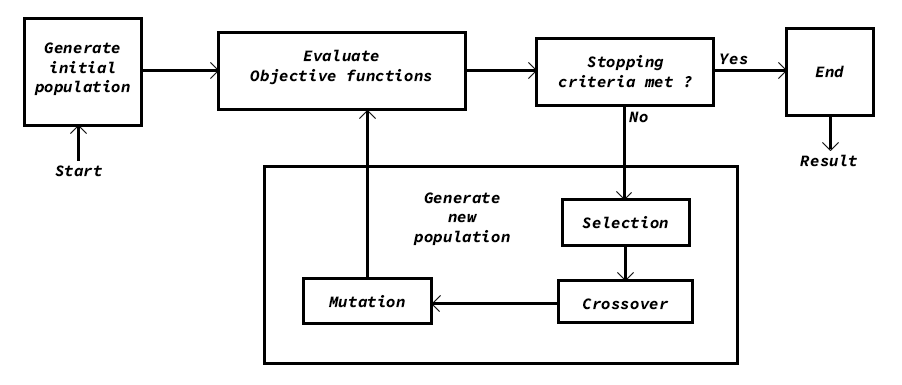
\includegraphics[width=0.8\textwidth]{img/ga_life_cycle.png}
    \caption{Ciclo de vida de un algoritmo genético}
    \label{figure:GA-Cycle}
\end{figure}

La lista anterior se muestra gráficamente en la Figura \ref{figure:GA-Cycle}, en
donde se puede apreciar más claramente como los operadores de selección, cruce y
mutación se engloban en una sola área que es la de la generación e integración
de nuevos individuos, éstos  también se evalúan para definir si el algoritmo ha
logrado alcanzar el punto de terminación, como
se explicó anteriormente estos nuevos individuos no se eliminan en caso de no
haber sido los ideales, sino que se comparan con los individuos originales y en
caso de ser mejores irán reemplazando a los peores con el fin de encaminar al
algoritmo a un punto especifico que se espera sea la solución idónea.

\section{Generación procedural de contenido}
\label{section:PCG}

El término "Generación procedural de contenido" (Procedural Content Generation o
PCG por sus siglas en inglés) denota la manera de crear contenido de manera
automática mediante algoritmos, en lugar de generar los mismos contenidos de
manera manual. %  Agrega referencias


La PCG es un sistema de generación de contenido utilizado desde finales de los
70s, inicialmente se utilizaba para generar los laberintos de algunos juegos
utilizando arte ASCII donde se denotaba la distribución de los cuartos y objetos
que se podían encontrar en juegos estilo \textit{"rogue"} 
o juegos que simulan %  Agrega referencias
un juego RPG de mesa, actualmente es ámbito de la generación de contenido ah
tomado varias variantes y cada vez más empresas toman un interés por el uso de
este tipo de herramientas de diseño, cabe remarcar que los diferentes ámbitos no
están del todo refinados sin embargo dada la información necesaria y aplicados a
aspectos específicos en el ciclo de desarrollo son capaces de crear los
contenidos que se requieran.

Mientras que la generación de contenido es un aspecto que se ha utilizado en
muchos ámbitos diferentes como en el fotografía, video, anuncios y arte digital, en
el área de videojuegos se maneja el uso de generación "procedural" de contenido
en donde procedural se define como el proceso computacional de una función
particular, en este caso lo que se busca con la generación procedural de
contenido es reducir el tiempo que toma generar contenidos de manera manual, la
siguiente sección explica más detalladamente como se utiliza esta mecánica en el
área de videojuegos.

\subsection{PCG en el ámbito de videojuegos}
\label{subsection:PCGInGames}

Dentro del ámbito de videojuegos la generación de contenido procedural es un
aspecto que ha tenido un gran impulso en tiempos recientes debido a que muchas
empresas de preocupan por sacar al mercado juegos de manera contínua, estos
mismos muchas veces en ciclos de desarrollos muy cortos, por lo mismo, se han buscado
diferentes maneras de reducir dichos problemas. Una herramienta útil que ha
surgido debido a esto es la generación procedural la cual permite reducir no
solo los tiempos de desarrollo, sino que también permite recudir el espacio de
memoria total de un juego en particular debido a que ya no es necesario tener
todos los archivos englobados en un solo lugar, sino que lo requerido se obtiene
de manera automática, de esta misma manera se les permite a las empresas reducir
el número de personal necesario y por tal reducir los costos de desarrollo.

La generación procedural de contenido tiene tres objetivos %% Referencias Según X la ..
principales:
\begin{itemize}
    \item Brindar apoyo a los creadores para poder crear contenido mas
    rápidamente.
    \item Utilizar la generación de contenido para crear juegos que logrean
    reaccionar en tiempo real a las acciones de los usuarios, cosa que en caso
    contrario tendría que encaminarse a escenarios específicos.
    \item Reducir el espacio en memoria tomado por el contenido generado.
\end{itemize}
Una cosa extra que brinda la generación procedural de contenido es permitir una
mayor creatividad al momento de generar.

\subsection{Áreas de interés de generación procedural}
\label{subsection:PCGAreasOfInterest}

La generación procedural de contenido es un sistema que se enfoca en diferentes
aspectos en el área del entretenimiento especialmente en el área de videojuegos,
estos aspectos pueden o no estar ligados unos con otros y además cabe mencionar
que no se enfocan primordialmente en la generación de "objetos" sino más bien en
la generación de recursos que pueden ser utilizados en el desarrollo de
videojuegos, la generación procedural se enfoca en seis puntos mostrados en la
Figura \ref{figure:pcg_areas}, cada uno se explica en un apartado iniciando con
el 'Diseño de niveles' en el capítulo \ref{subsection:LevelDesign}, la
generación de gráficos en el capítulo \ref{subsection:Visuals}, la creación de
audio en el capítulo \ref{subsection:Audio}, creación de narrativa o historias
en el capítulo \ref{subsection:Narrative}, diseño de reglas y mecánicas en el
capitulo \ref{subsection:rulesandmechanics} y la generación de juegos completos
explicada en el capítulo \ref{subsection:games}.

\begin{figure}
    \centering
    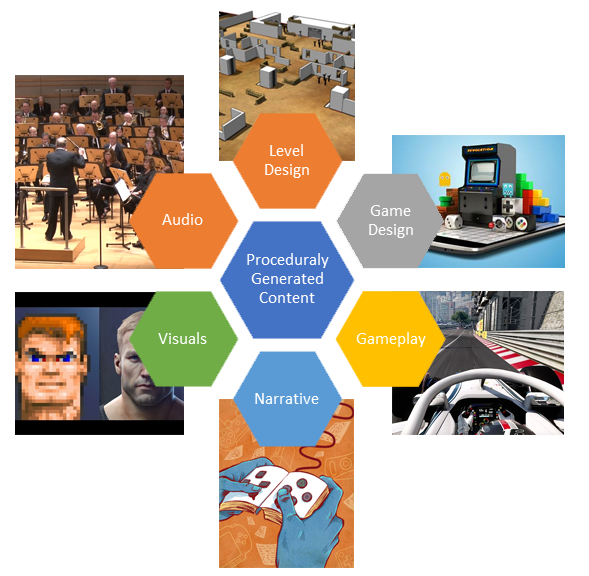
\includegraphics[width=0.6\textwidth]{img/pcg_areas.png}
    \caption{Áreas de PCG en videojuegos}
    \label{figure:pcg_areas}
\end{figure}

\subsection{Diseño de niveles}
\label{subsection:LevelDesign}

El área del desarrollo de niveles es una de las populares en PCG debido a que
los niveles son la parte esencial de un juego, debido a que es el área sobre la
cual un jugador puede interactuar, la representación de estas áreas pueden ser 
desde imágenes en 2D, simplemente con el alto y ancho de los objetos, hasta
elementos en 3D que abarquen también el grosor de los objetos.

Debido a que los niveles son esencialmente el área principal de interacción en
un videojuego, éstos deben de considerar los aspectos de funcionalidad y estética
para que exista una buena interacción y sea llamativo a los usuarios, de esta
manera se pueden crear áreas con tonos oscuros y ambiente tétrico para entregar
un nivel con temática de terror. La generación de niveles de juego es un tema
reciente en el ámbito de investigación debido a los elementos que se deben de
tener en cuenta sin embargo dentro del ámbito de videojuegos, es un elemento
comúnmente utilizado, algunos ejemplos recientes siendo Spelunky, Minecraft y
Disgaea. %% urls o referencias

Primero tenemos el juego de plataforma Spelunky desarrollado por Derek Yu, el
juego consta de múltiples niveles alrededor de cinco diferentes áreas, cada área
con un estilo diferente (niveles con hielo, lava, etc.) en este juego los niveles
que recorre el jugador son desarrollados de manera procedural por diferentes
algoritmos dependiendo el área en la que se encuentre el jugador.%% urls o referencias

El segundo ejemplo es un videojuego desarrollado por Markus Persson llamado %% urls o referencias
Minecraft, este juego consta de un área estilo caja de arena en donde el jugador
puede realizar las acciones que quiera, las estructuras están definidas en
manera de bloques con diferentes texturas y propiedades que el jugador puede
utilizar para construir diferentes cosas, la manera en cómo se utiliza la
generación de contenido es mediante la generación de todo un nivel al iniciar el
juego de tal manera que se utiliza una semilla de generación y se utiliza el
método \textit{Perlin Noise} 3D con interpolación lineal para generar los biomas,
elementos y entidades que conformaran el nivel, además de esto el área inicial
del juego no es la única área que puede ser recorrida durante la sesión de
juego, sino que el sistema utiliza una "semilla"(seed) que define la manera en
cómo está conformado el mapa, mientras más se va recorriendo del mapa las áreas
se van generando acorde a la semilla de manera infinita.

Finalmente tenemos el juego Disgaea desarrollado por Nippon Ichi Software, este %% urls o referencias
es un juego de estrategia por turnos en donde el objetivo es eliminar a todos
los enemigos en un mapa para continuar al siguiente, la manera en cómo se
utiliza la generación de contenido procedural es en una sección extra del juego
en donde se puede entrar a un arma para completar niveles gradualmente mas
difíciles para darle más poder a dicha arma, en esta parte los niveles que se
encuentra el jugador son generados proceduralmente tomando en cuenta las alturas
de las partes donde se puede caminar y la colocación de los enemigos en el mapa
\ref{figure:DisgaeaIW}, para la generación se toma en cuenta el nivel del arma y
su rareza, mientras más altos sean estos valores de igual manera los niveles
generados serán más difíciles.

\begin{figure}
    \centering
    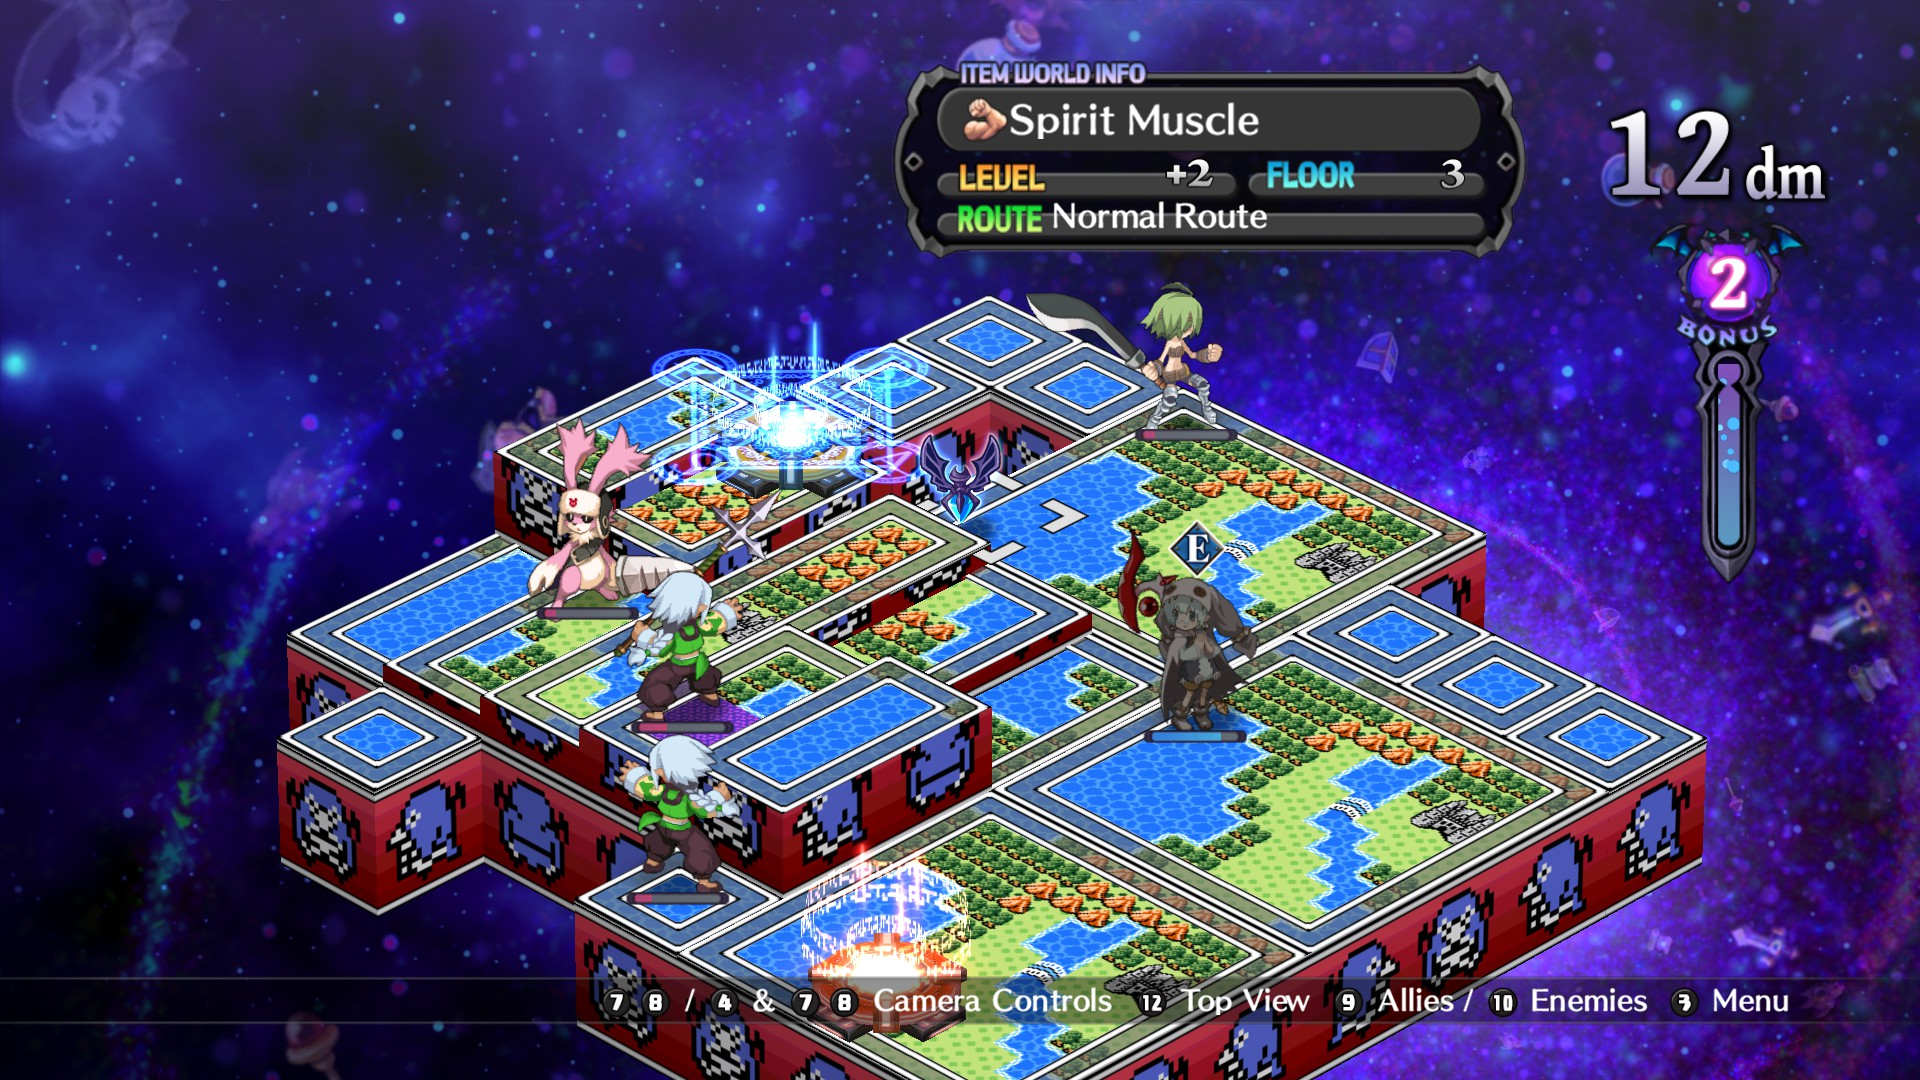
\includegraphics[width=1.0\textwidth]{img/DisgaeaIW.png}
    \caption{Nivel generado en el juego Disgaea}
    \label{figure:DisgaeaIW}
\end{figure}

\subsection{Gráficos}
\label{subsection:Visuals}

El área de desarrollo de gráficos se encarga principalmente de generar las
representaciones visuales de los juegos debido a que la mayor parte de los
juegos llevan una parte visual a menos que no se requiera, es necesario generar
una imagen que denote lo que se quiere dar a entender en un juego, de esta
manera se le brinda al jugador un nivel más de inmersión en la situación,
mediante el uso de paletas de colores o imágenes en pantalla que puedan
representar mejor las situaciones que se presentan.

El ámbito de generación de gráficos ha sido uno de los más explotados debido a
que es posible generar gráficos que van desde simples representaciones de 8 bits a
representaciones foto realísticas de los eventos u objetos presentes en un
juego. Tal es el caso explicado en el paper de Risi S. et al.\cite{Risi2012} en
donde utilizan una red de producción de patrones composicionales (CPPN por sus
siglas en inglés) la cual es una variante de las redes neuronales artificiales
(ANN) regulares, utilizando esta red se buscó modificar un círculo de tal manera
que la resultante de tal modificación creara un patrón en forma de una flor, de
igual manera la forma de crear diversidad en los tipos de flores generadas fue
mediante el uso de la neuro evolución de topologías aumentativas (NEAT) mediante
el cual las redes generadas se alteraban mediante la modificación de conexiones
entre neuronas y la adición de nuevos nodos de tal manera que se buscaba un
nivel adecuado de complejidad para las redes que generaron diferentes tipos de
patrones de flores.

Mientras que un segundo artículo escrito por Erin J. et al.\cite{Hastings2009} en
el cual presentan un nuevo algoritmo de generación de contenido llamado
neuro evolución de topologías aumentativas para generación de contenido (cgNEAT)
el cual se encarga de generar contendió gráfico y contenido del juego de acuerdo
a las preferencias de un jugador mientras el juego está en ejecución, para la
evaluación del contenido generado se desarrolló un juego multijugador en línea
llamado \textit{Galactic Arms Race} en el cual la cgNEAT se encarga de generar
contenido para todos los jugadores y ellos eran quienes proveían la
retroalimentación del funcionamiento del algoritmo.

\subsection{Audio}
\label{subsection:Audio}

El ámbito de generación de audio en videojuegos se puede considerar como un
punto opcional dependiendo del juego que se esté desarrollando sin embargo el
audio juega un papel importante en la experiencia que se le brinda a un jugador
dentro del juego debido a que mediante el uso de componentes sonoros se pueden
influir las emociones que se quieren mostrar en lugares específicos, desde cosas
simples como el uso de sonidos de objetos como escuchar un teclado siendo
utilizado hasta la utilización de pistas de audio en áreas o momentos clave del
juego para demostrar momentos dramáticos, tristes o de acción. 

Cabe mencionar que es posible utilizar instrumentos musicales o la
implementación de orquestas para de igual manera generar estos ambientes sin
embargo algunos utilizan este tipo de generación para crear pistas que sean
capaces de adaptarse a los sucesos que transcurren en el momento para el
concepto de generación procedural de audio puede ser inclusive el uso de
elementos en un entorno virtual que generen algún sonido cuando son
interactuados \cite{garner2014sonic}, algunos ejemplos de adaptabilidad de audio
de acuerdo a los eventos en el momento es el caso del juego \textit{Fire emblem
Fates}, este es un juego de estrategia por turnos en donde la adaptabilidad de
audio se da en transiciones de vista del mapa y combate de unidades, en este
caso el audio de la vista del mapa tiene un cierto nivel de \textit{tempo}
mientras que en momento que se entra a un combate entre dos unidades el
\textit{tempo} del audio cambia mientras se está en esta escena de combate.

Existen también investigaciones académicas de como combinar la generación de
niveles con la generación de audio, tal es el caso de \textit{Sonancia}
desarrollado por Phil Lopez et al. \cite{lopes2015sonancia}, en este paper los
autores proponen una metodología que permitirá a un sistema generador de niveles
seleccionar pistas de audio o sonidos que vallan de acuerdo a un tema específico,
en este caso los autores colocaron una lista de pistas y mediante un generador
crearon un entorno 2D que simulaba una mansión, el propósito fue el de crear un
juego de terror/suspenso y que las habitaciones tuvieran un audio diferente y
que al acercarse a la división entre una y otra el audio de la habitación
adyacente fuese subiendo el volumen conforme más se adentraba y el audio de la
habitación anterior se dejará de escuchar lentamente, el sistema es capaz de
generar los niveles y asignar los sonidos necesarios sin embargo tiene la
limitante de que se debe de proporcionar el listado de pistas de audio debido a
que aún no tiene la capacidad de generar audio por cuenta propia sin embargo es
otro buen ejemplo de cómo combinar áreas de generación de contenido.

Otro caso de estudio es el del juego \textit{Audio Surf} desarrollada en 2008 por
Fitterer, la manera en cómo funciona es que mediante el uso de archivos de audio
de alguna canción para generar niveles estilo pista de carreras que el usuario
recorre al momento de jugar, como este existen varios otros juegos que utilizan
mecánicas de PCG para generar los niveles a jugar por los participantes.

Finalmente tenemos \textit{Mezzo} desarrollado por Daniel B. este artículo muestra
un programa de computadora del mismo nombre diseñado con el fin de generar
música de la era romántica que puede ser utilizada en juegos de computadora, el
software fue desarrollado con el propósito de poder darle más expresividad a
eventos que ocurren en juegos de computadora, esto es mediante el uso de los
elementos presentes en la escena como las partes que conforman la pieza musical,
para esto sus acciones son traducidas como diferentes cantidades de tension
armónica lo cual permite que la pieza musical corresponda al estado del juego
así como a las acciones que realizan los personajes.

\subsection{Narrativa}
\label{subsection:Narrative}

El ámbito de generación de narrativa en videojuegos se encarga de manera básica
de generar historias que tengan sentido y sean entretenidas, el uso de PCG para
el ámbito de narrativa se ha tomado de diferentes ángulos, el primero es
sencillamente crear la historia del lugar en donde se desarrollan las cosas,
esto es generar toda la historia desde un punto especifico y así crear una
"línea" de acción que un jugador deberá seguir, mientras que otro de los
aspectos es la generación de historia que se adapte a las acciones del jugador,
esto es, que a medida que el jugador progrese en un juego realizando acciones
especificas el juego adapte la historia a generar de acuerdo a dichas acciones.

Algunos ejemplos de este ámbito de generación se muestran en el juego
\textit{Facade} y el sistema \textit{Versu}, el primero que se explicara es el
juego de Facade, Facade es un juego desarrollado por Michael Mateas y Andrew
Stern \cite{mateas2003faccade} que intenta crear un juego estilo novela visual
en donde las acciones del jugador tengan influencia en los eventos que ocurren
en el juego, el juego introduce al personaje del jugador como un amigo de una
pareja de casados, no se cuenta con un objetivo específico más que el de
completar la historia, sin embargo, el juego provee de acciones y respuestas que
el personaje puede expresar a la pareja, estas mismas tienen influenciaran
directamente el cómo se desarrollará la historia, el juego se diseñó con el
propósito de que el jugador lo repita múltiples veces con el fin de descubrir
como las diferentes decisiones cambiaran el desenlace de la historia. 

Finalmente \textit{Versu} es una aplicación desarrollado por Richard Evans y
Emily Short \cite{evans2013versu} es juego se encarga de generar simulaciones en
base a líneas de texto que denotan acciones que un conjunto de personajes no
jugables (NPC) realizan en determinados escenarios, el juego permite que a una
persona se le asigne un personaje del juego y controle las acciones que
realizara, mientras que los NPC restantes responderán de manera autónoma
mientras el juego continua, este sistema de generación de narrativa inicio como
un proyecto académico y después paso a ser utilizado de manera comercial, además
de ser la base para el desarrollo de otros juegos de estilo similar.

\subsection{Reglas y Mecánicas}
\label{subsection:rulesandmechanics}

Las reglas y mecánicas de un juego proveen un framework en el cual el
jugador puede realizar acciones y el cómo debe de influenciarlas hacia un
objetivo final, las reglas y mecánicas de un juego pueden variar dependiendo del
tipo de juego que se trate, por ejemplo, en juegos de estilo plataforma la regla
de terminación puede ser simplemente llegar hasta cierto punto del nivel
mientras que las mecánicas pueden incluir saltar, correr o agacharse, este
conjunto de reglas permite que el jugador no realice acciones no previstas por
los programadores y de tal forma limita a un jugador a cierta cantidad de
acciones y consecuentes posibles las cuales deberá de aprovechar de diferentes
maneras para continuar.

Mientras que el uso de reglas permite tener un juego más balanceado algunas
ocasiones el cambiar el conjunto de reglas permite crear diferentes tipos de
juegos, tomando el ejemplo anterior es posible que un juego de plataformas se le
permita a un jugador volar en un nivel lo cual provocaría que las mecánicas se
requieran acomodar a esta nueva habilidad y de igual manera los niveles de un
juego se tengan que re-imaginar de tal modo que ahora se pueda utilizar en
ciertas o se coloquen lugares que solo se pueden acceder con esa habilidad por
ejemplo la transición de reglas y mecánicas entre los juegos Super Mario Bros.
(Nintendo, 1985) y Super Mario World (Nintendo, 1990). %Referencias

Para la evaluación de la generación de mecánicas y reglas de un juego existen
diferentes métodos a utilizar, el primero se basa en el balance de las reglas es
decir en caso de ser un juego para dos o más jugadores el objetivo de evaluar
sería que todos los jugadores tengan las mismas probabilidades de ganar
utilizando las mecánicas del mismo juego, mientras que otra manera de evaluar
seria mediante la facilidad que tienen las mecánicas de ser aprendidas por los
jugadores.

En cuanto a ejemplos de este tipo de generación se encuentran algunas
investigaciones académicas tales como la de Ludi \cite{Browne2010}, Ludi es un
sistema desarrollado por Cameron Browne y Frederic Maire, este sistema se
utiliza para evolucionar comandos que definen las reglas de un juego en
particular a crear, el algoritmo evolutivo se encarga de evolucionar las reglas
manteniéndolas dentro de un cierto rango de métricas que establecen un buen
patrón para juegos de tablero tales como tales como la complejidad del juego o
la simplicidad de las reglas, un juego de mesa diseñado mediante el uso de este
sistema se llama Yavalath, una vista rápida del juego se puede apreciar en la
figura \ref{figure:Yavalath}, este juego puede tener un mínimo de 2 y un máximo
de 3 jugadores, las reglas son que en base a turnos cada jugador coloca una
ficha de su color en cualquier punto no ocupado del tablero, el objetivo es
lograr formar una línea de 4 fichas del mismo color, pero la regla es que al
formar una línea de 3 fichas se pierde el juego de manera automática, de esta
manera el juego se basa en forzar jugadas del oponente que permitan que alguno
tenga más "control" de los eventos que ocurrirán. 

Un segundo caso fue escrito por Togelius et al. \cite{Togelius2008}, este uno de
los primeros ejemplos del uso de computación evolutiva para la generación de
reglas para juegos, en este paper se evoluciona un conjunto de reglas de tal
manera que un conjunto de agentes que participaran en el juego logren tener un
mejor entendimiento de como funciona el juego, la manera de evaluar que tan
entendibles son las reglas fue a través de varias sesiones simuladas de los
agentes, en este caso se procuró utilizar reglas sencillas que simularan un
juego estilo pac-man en donde los agentes deberían de colectar círculos para
poder obtener una mejor puntuación.

Finalmente, un último caso es el de Nielsen et al. \cite{Nielsen2015} esos
autores programaron un sistema capaz de representar las reglas de un videojuego
utilizando video game description language en donde juegos estilo 2d se
representan como mapas en base a caracteres y utilizaron ASP para verificar que
los niveles podían ser jugados (se podían cumplir las condiciones de victoria).

\begin{figure}
    \centering
    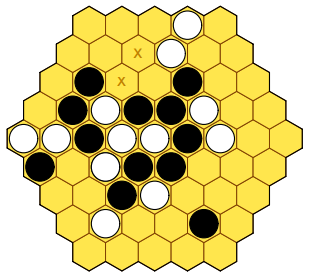
\includegraphics[width=0.6\textwidth]{img/Yavalath.png}
    \caption{Ejemplo de un juego en progreso en el juego de Yavalath}
    \label{figure:Yavalath}
\end{figure}

\subsection{Juegos}
\label{subsection:games}

Mientras que las facetas de generación anteriores se han enfocado en aspectos
específicos de juegos mientras que en este aspecto en particular se toma un
enfoque global, esto es desde la generación de partes visuales hasta la 
generación de bandas sonoras, esto demuestra como todos los aspectos de un
juego se relacionan unos con otros, un ejemplo de esta relación seria tomar un
juego en particular y agregar acciones que originalmente no existían, para poder
agregar estas acciones se debe de considerar el aspecto visual, es decir el como
deberá de representarse visualmente tal acción, aspectos de sonidos en caso de
que una acción requiera de algún efecto de sonido que represente tal acción,
utilizando el ejemplo de agregar la mecánica de volar, el aspecto visual se
representaría en un cambio visible en el personaje controlado, por ejemplo,
dibujar alas y que se vea una animación de movimiento al volar, en el caso del
aspecto del sonido el aleteo o movimiento generado por dichas alas al estar
volando puede tener un sonido único para identificarlo.

Para este caso existen diferentes maneras de intentar generar juegos nuevos, tal
es el caso de Game-O-Matic \cite{treanor2012game}, Game-O-Matic es una
herramienta de generación enfocada a la generación de juegos que representan
ideas, en este sistema se utiliza un sistema de sustantivos unidos mediante
verbos que son ingresados al sistema como datos de entrada, estos datos son
procesados y se logra generar un juego simple estilo arcade que logre
representar un mapa conceptual generado mediante los valores de entrada. 

Otra investigación realizada por Nelson et al. \cite{Nelson2008}, para este
sistema los autores proponen un sistema parecido al de Game-O-Matic explicado
anteriormente, sin embargo, en este caso el sistema está basado en sprites que
representan entidades del juego, lo que se asigna como valor de entrada es
restricciones que definen la interacción de los sprites en pantalla, las
restricciones son procesadas mediante una red semántica y una base de datos de
léxico, este proceso logra generar juegos que cumplan las restricciones
estipuladas, en este caso los juegos generados tienen mecánicas estilo WarioWare
en donde los juegos tienen una regla de victoria sencilla que hace los juegos
relativamente cortos. 

Finalmente, uno de los mejores generadores de juegos lleva en nombre
de ANGELINA \cite{cook2011multi} %(Ref ANGELINA num135-137) 
\footnote{De acuerdo al autor: "A Novel Game-Evolving Labrat I've Named
ANGELINA"}, ANGELINA es un sistema de generación de juegos diseñado
originalmente en 2011 y que ha recibido modificaciones desde entonces, la base
del generador es el uso de un sistema evolutivo que se encarga de evolucionar
las reglas, los terrenos, los personajes y demás conjuntos con respecto unos de
otros de una manera orquestada, se encarga no solo de evolucionar la
información visual de los componentes sino también de asignar sus locaciones en
un campo de trabajo que representa un juego, además de esto es capaz de
seleccionar elementos musicales relevantes al tema de los mapas generados o de
la faceta emocional presente en el juego además de crear asignarle un nombre a
los juegos que logra crear, inicialmente el sistema era capaz de generar niveles
de plataforma en 2D, pero actualmente es capaz de generar niveles de temática de
aventura en entornos 3D.

Los anteriores generadores a pesar de no ser perfectos han permitido dar un gran
paso en la generación de contenido o más bien en la generación de juegos, sin
embargo aún falta controlar aspectos que permitan que las generaciones de tal
contenido logren involucrar todos los aspectos de la generación de contenido,
esto podría darse mediante el uso de múltiples agentes que contantemente evalúen
los aspectos generados pero que al mismo tiempo logren comunicarse unos con
otros y poder evaluar los juegos generados de manera más amplia.

\section{Jugabilidad}
\label{section:playability}

La jugabilidad es un término utilizado principalmente en el área del análisis y
diseño de videojuegos y es utilizado principalmente como medida de calidad para
la experiencia de un usuario para con el juego mediante las mecánicas o manera
en cómo se tiene una interacción jugador-videojuego y el diseño como tal del mismo.

De igual manera diferentes autores definen el concepto como un conjunto de
propiedades que definen la experiencia que logra tener un jugador en un juego
determinado según al sistema de juego que se provee.

\begin{figure}
    \centering
    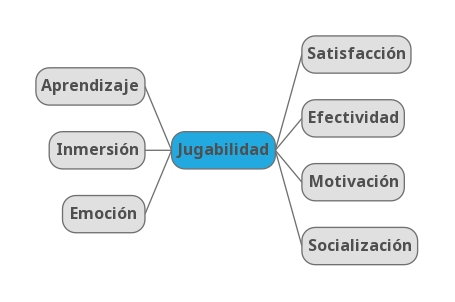
\includegraphics[width=0.7\textwidth]{img/playabilityv2.png}
    \caption{Puntos de evaluación de jugabilidad}
    \label{figure:playability}
\end{figure}

La figura \ref{figure:playability} muestra un diagrama de áreas y conceptos que
califican el nivel de jugabilidad de una aplicación o juego, estos mismos se
pueden definir como sigue:

\begin{itemize}
    \item Satisfacción: El grado en el que un juego logra agradar o complacer a
    un usuario.
    \item Aprendizaje: El grado con el cual un usuario es capaz de comprender
    las mecánicas de un juego y es capaz de interactuar fácilmente con el mismo.
    \item Efectividad: Este demuestra la cantidad de recursos y el tiempo
    utilizados para poder envolver a un usuario y lograr que se divierta.
    \item Inmersión: El grado con el cual se logra envolver a un usuario con los
    eventos que transcurren en el juego, es decir que tanto se logra hacer que
    se integre o muestre empatía por los eventos del juego.
    \item Motivación: Esta define la capacidad que tiene un juego a motivar a un
    usuario a continuar con los retos o eventos del juego, esto generalmente se
    da por mecánicas que dan un sentimiento de recompensa o simplemente por la
    inmersión lograda.
    \item Emoción: Es el grado con el cual se logra una inmersión en el usuario
    de tal manera que es capaz de reaccionar de manera involuntaria a estímulos
    presentados en el juego, esto puede ser desde una risa por algún evento que
    ocurre hasta saltos involuntarios por susto en juegos de terror.
    \item Socialización: Este es el grado con el cual se logra que un usuario
    entable relaciones con personas que no conoce, en juegos de multijugador
    masivo en línea("Massive-Multiplayer Online" - MMO por sus siglas en ingles)
    existen eventos en los cuales se le pide a los usuarios que construyan
    equipos para completar niveles en el juego, existen otros juegos de
    multijugador local en los que varias personas compiten para ganar, y en
    ambos casos se puede presentar que de los sucesos presentados se puedan
    crear amistades entre jugadores.\cite{sanchez2009playability}
\end{itemize}

Por otro lado, existe un conjunto de facetas que engloban varios atributos de la
jugabilidad que permiten relacionar dichos atributos, para estas facetas se
toman los siguientes grupos:

\begin{itemize}
    \item Jugabilidad intrínseca: Engloba el diseño y mecánicas del juego
    enfocándose en las reglas y objetivos establecidos, define el cómo se
    proyectan estos puntos al jugador.
    \item Jugabilidad mecánica: Se enfoca en parte funcional del juego y en los
    comportamientos de los personajes, se basa en el diseño del motor del juego.
    \item Jugabilidad interactiva: Se enfoca más en la relación usuario-juego,
    tomando en cuenta el cómo se presenta la interfaz de usuario y los controles.
    \item Jugabilidad artística: En este punto se engloban los puntos de
    gráficos y sonido, es decir que tan bien es visualmente lo que se presenta y
    el tipo de ambientación que se crea al combinar efectos visuales, música y gráficos.
    \item Jugabilidad perceptiva: Este punto trata de cuantificar la manera en
    como una persona percibe los elementos mostrados en el juego, este es un
    calculo subjetivo.
    \item Jugabilidad interpersonal: Al igual que el punto anterior es un
    concepto subjetivo, sin embargo, este se enfoca en las percepciones que se
    generan al jugar en un grupo.
\end{itemize}

\section{Open-Ended Evolution}
\label{section:open-ended_Evolution}

El termino Open-Ended Evolution (OEE) es el nombre que se le da a una variante
del algoritmo de evolución genética, este algoritmo difiere de los objetivos
predefinidos de un algoritmo genético en el cual el objetivo principal de un GA
es el de llegar o aproximarse a un valor o conjunto de valores que logren
solucionar un problema determinado, en el caso de OEE este no es el caso sino
que lo que hace el algoritmo es seguir evolucionando y creando diversidad en la
población cada vez más compleja no solo dentro de los límites de evolución de un
elemento sino comenzar a crear nuevas \textit{"especies"} de soluciones.

Una explicación más clara es presentada en un paper por T. Taylor et
al.\cite{Taylor2016}, en este paper se define OEE como un sistema capaz de
novedad después de un punto en la evolución en donde el estado del grupo o
población no cambia en lugar de converger hacia un estado casi estable.

La manera en cómo se definirá el uso de OEE que se utilizara en este proyecto es
simplemente un proceso de evolución genética capaz de encapsular procesos de
evolución similares capaces de incrementar en número según la complejidad a la que
las entidades generadas logren llegar.
